\section{Matched optimization study}\label{sec:optimization}
This section tests whether adjoint-driven optimization shortens the time
needed to reach a common validated ripple target. The protocol and all of
its amendments were fixed in the
\href{https://github.com/rjwalters/geode-fem/issues/1185}{preregistration}
before any main-run outcome was observed. One later deviation, in how the
final refinement was run, was adopted after the main runs had finished and
is described in the \emph{Final refinement} paragraph of
Section~\ref{sec:exp2-results}; it changes no selection rule, check or
target.

\subsection{Protocol}
\paragraph{Coarse and validation simulations.}
The optimizers never query the simulation that scores them. Each queries a
\emph{coarse simulation}, the L1 mesh (the coarser L0 for methods D and E)
with interface order 45, and its search is driven only by coarse values.
Every design that becomes the method's new best, its incumbent, is rescored
on one \emph{validation simulation}, the finer L2 mesh with interface order
93, which no optimizer sees; only validated scores count toward a target.
Both are physics simulations, the nonlinear finite-element model of
Section~\ref{sec:model} at two mesh levels and interface orders, neither
fitted to torque data nor corrected against validation; of what the
optimizers use, only their own search models, C's radial-basis surrogate
and COBYQA's interpolation model, are fitted, to coarse values.
Validation is charged to the run that requests it, as in a
design loop that must check its candidates before trusting them; this
validate-every-incumbent rule costs methods that change incumbents often
the most, and Section~\ref{sec:exp2-results} reports its share of each
run's time.

\paragraph{Methods.}
Five methods form an optimizer-by-resolution comparison plus one
surrogate (Table~\ref{tab:methods}). A and E are SLSQP
\citep{kraft1988} using the field adjoints of Section~\ref{sec:gradients},
safeguarded so that a refused request restores the last admissible point
and restarts the solver; B and D are COBYQA \citep{ragonneau2022} with $2n+1$ interpolation points
and unit-box trust radii $0.1$ to $10^{-6}$, where $n$ is the number of free
parameters. Both run through SciPy 1.18.1 \citep{virtanen2020scipy}. C is
an empirical trust-region method on four cubic radial-basis interpolants
of the L1 coarse outputs (the three per-current standard deviations and
the full-current mean), refitted after every evaluation from an $n+1$-point
initial design; Appendix~\ref{sec:settings} gives its radii, acceptance
and update rules and the other settings. B against A and D against E vary
the optimizer at fixed coarse resolution, and E against A and D against B
vary resolution at fixed optimizer; every paired ratio below is written in
this order (B/A, D/E, E/A, D/B), so a value above one favors the second
method. The optimizer contrast
changes the search strategy and the gradient source together;
Section~\ref{sec:exp2-fd} separates them with the three further methods of
Table~\ref{tab:methods}. The coarse simulation uses order-45 coupling torque
on 20 angles at current fractions $0$, $\tfrac12$ and $1$ of the fixed peak
current $9.6777\,\mathrm{A}$. L0 and L1 differ only in spatial resolution.
Time to a fixed
target, with unattained targets kept as censored, follows the data- and performance-profile
practice for benchmarking optimization solvers \citep{more2009benchmarking,dolan2002benchmarking}.
The preregistration also named a fixed group-1 current-density rule as a
labelled control. It was not run in this study, which uses the fixed
physical current throughout; Section~\ref{sec:gradients} reports that
rule's effect on sensitivities.

\begin{table}[H]\centering\small
\caption{Methods. A--E form the preregistered study (two repeats each).
FD-cold, FD-warm and A$'$ form the post-hoc ablations of
Section~\ref{sec:exp2-fd}; each ablation ran in its own session with A
rerun unchanged as A$'$.}
\label{tab:methods}\setlength{\tabcolsep}{5pt}
\begin{tabular}{llll}\toprule
Method & Optimizer or search model & Gradient & Coarse simulation\\\midrule
A & Safeguarded SLSQP & Field adjoint & L1\\
B & COBYQA & None & L1\\
C & Empirical cubic-RBF trust region & None & L1\\
D & COBYQA & None & L0\\
E & Safeguarded SLSQP & Field adjoint & L0\\\addlinespace
FD-cold & Safeguarded SLSQP & Forward differences, cold stencils & L1\\
FD-warm & Safeguarded SLSQP & Forward differences, warm stencils & L1\\
A$'$ & A, rerun in each ablation & Field adjoint & L1\\\bottomrule
\end{tabular}
\end{table}

\paragraph{Design spaces and constraints.}
The 8-parameter space S8 frees eight geometric lengths: MAG, MH, MW,
SW1--SW4 and Sr1 (Fig.~\ref{fig:geometry}a,b), that is, the rotor iron
depth, magnet height and width, four stator tooth and slot dimensions, and
the slot-bottom fillet radius. The 18-parameter space S18 adds the ten
grouped offsets of Fig.~\ref{fig:geometry}c, which move 55 control points
of the rotor surface and the stator bore. Stack length, radial scale,
stator outer diameter and operating angle are fixed, so the saved Opt120
design lies outside both spaces. Table~\ref{tab:paramsets} compares these
spaces with the 12-parameter set whose gradients Section~\ref{sec:gradients}
verifies. The two spaces also use different discrete mesh-motion maps, so
their contrast does not isolate the ten added offsets.
Each coarse simulation $r\in\{\mathrm{L0},\mathrm{L1}\}$ minimizes
$F_r=\sum_c\sigma_{r,c}^2$ over the three objective currents $c$, subject to
$\bar T_{r,1}\geq1.0025\,\bar T_{r,1}(\theta_0)$ for its own full-current mean and to
normalized construction margins $c_i-0.05\geq0$. Here $\theta_0$ is the
reference's published initial design. Unbuildable or
mesh-infeasible candidates are refused: SLSQP restores toward the last
admissible point and restarts, COBYQA receives a NaN barrier, and C skips
the point. A moved mesh with an inverted triangle or a minimum angle below
$5^\circ$ is repaired by up to four charged remeshing attempts. Because
refinement cannot remove a limiting geometric corner, the $5^\circ$ policy
also acts as an implicit geometric constraint. S18's slot-opening
channel wall is not guarded and can become very thin at extreme offsets;
that risk is handled by repair and refusal, not by a wall-thickness
constraint.

\begin{table}[H]\centering\small
\caption{The three parameter sets. Section~\ref{sec:gradients} verifies
the gradients of a 12-parameter scalar set; the optimizers search S8 and
S18, whose gradients are checked separately
(Appendix~\ref{sec:protocol-details}). Values are in
Table~\ref{tab:parameters}.}
\label{tab:paramsets}
\begin{tabular}{llll}\toprule
Parameters & Gradient check (12) & S8 & S18\\\midrule
MAG, MH, MW (magnet) & free & free & free\\
SW1--SW4, Sr1 (stator slot) & free & free & free\\
SD1, axial length, $\phi_0$, radial scale & free & fixed & fixed\\
CPR1--CPR7, CPS1--CPS3 (offsets) & --- & --- & free\\\bottomrule
\end{tabular}
\end{table}

The gradients A and E use, including those of S18's grouped offsets,
agree with central differences in both spaces within $2.8\times10^{-7}$
relatively in the directional checks (Appendix~\ref{sec:protocol-details}).

\paragraph{Common validation and credit.}
Every method is judged on the same order-93, L2, 20-angle validation simulation.
Its initial-design anchor is $F_0=9.6034\times10^{-3}\,\mathrm{N^2\,m^2}$ with
full-current mean $\mu_0=1.44084\,\Nm$. Target $T_x$ is an $x$\% reduction
of $F_0$: $T_{50}=0.5F_0$, $T_{90}=0.1F_0$ and $T_{99}=0.01F_0$. The
\emph{primary targets} are $T_{90}$ in S8 and $T_{99}$ in S18, the deepest
target reached in each space (no run reaches $T_{99}$ in S8). A validated
design is credited, and attains a target, only if
\begin{equation}
 F_{\mathrm{val}}+\delta F\leq T,\qquad
 \delta F=\max\{0.10F_{\mathrm{val}},\,2.5\times10^{-7}\,\mathrm{N^2\,m^2}\},
\end{equation}
its validated full-current mean is at least $1.0025\,\mu_0$, its
construction margins and mesh checks pass, and its validation completes
within budget. The allowance $\delta F$ is an empirical margin, not a bound
on continuum error. Optimizer success flags confer no credit. Changed
incumbents are validated as they appear, after the initial interpolation
set for B, C and D. A run's \emph{target crossing} is its first validated
design that attains the target; the time to the target is the charged time
at which that validation completes.

\paragraph{Budget, timing and cost vocabulary.}
Cost is wall time, in units of the median cold validation forward measured
on the same host at the same concurrency (66.66--70.94\,s in the three
sessions). A \emph{forward} is one evaluation of the objective: 60
nonlinear field solves, one per current fraction (3) and rotor angle (20).
In a \emph{cold} forward, Newton starts from zero at the first angle of each
current and from the previous angle's solution after that; in a
\emph{warm} forward, used only by FD-warm's stencils
(Section~\ref{sec:exp2-fd}), every field solve starts from the base
point's converged field at the same current and angle. A
finite-difference gradient adds one \emph{stencil solve}, a coarse
forward at a perturbed point, per parameter. Table~\ref{tab:costs} gives
what each operation costs in this unit. Each run receives 120 units,
with a 60-unit checkpoint that counts only validations completed by then.
The charge covers evaluator start-up, geometry checks, mesh motion and
repair, coarse forwards, adjoints, optimizer overhead, surrogate fitting
and validation; nothing is subtracted as overhead. L0 receives no discount.

\begin{table}[H]\centering\small
\caption{Cost vocabulary: medians of the recorded charges, in units of
the session's cold validation forward. The validation charge is that of
the 3,350 completed validations of the main study; the other rows are
from the ablation sessions (Section~\ref{sec:exp2-fd}), for $n=8$ and
$n=18$ parameters.}
\label{tab:costs}
\begin{tabular}{lll}\toprule
Operation & Simulation & Cost (units)\\\midrule
Validation forward & L2, order 93 & 0.87 (range 0.55--1.10)\\
Coarse forward & L1, order 45 & 0.216--0.245\\
Adjoint gradient, all $n$ components & L1, order 45 & 0.054--0.061\\
FD-cold gradient: $n$ cold stencil solves & L1, order 45 & 1.90 and 4.25\\
FD-warm gradient: $n$ warm stencil solves & L1, order 45 & 0.97 and 2.36\\\bottomrule
\end{tabular}
\end{table}

\paragraph{Starts and execution.}
Each space uses $\theta_0$ and four Latin-hypercube starts (LHS~1--4, seeds 1--4),
with the scalar coordinates matched across spaces. A start was eligible
only if it was buildable and admissible, and its moved reference mesh met
the mesh policy without repair, in both spaces at L0 and L1. The starts
therefore favor moderate deformations and are not uniform samples of the
design box. All starts were frozen before any main outcome. Every method
runs from every start twice, giving 100 runs. Within a start, repeat 1
rotates the method order and repeat 2 reverses it.

Each run is one single-threaded process; 15 ran concurrently on one AWS
c7a.4xlarge host, and all 100 completed in one session without recovery or
host contamination (Appendix~\ref{sec:protocol-details}).

\subsection{Results}\label{sec:exp2-results}
\paragraph{Repeats.}
The two repeats of each run follow the same optimization path. In all 50
pairs, the sequences of validated objectives agree exactly up to the
shorter run's length, and they differ in length only when the budget or a
solver stop cuts one repeat earlier. The repeats therefore measure timing
noise, not independent outcomes, and the comparison is a paired case study
over five starts. Over the 111 target crossings attained in both repeats,
the time differs by a median of 2.1\% and at most 12.4\% relative to
repeat~1. Repeat-1 times are reported below.

\paragraph{Attained quality.}
Figure~\ref{fig:exp2-quality} shows the best credited value of
$(F+\delta F)/F_0$ for every start, method and space (repeat~1).
In S8, no run goes below $F/F_0=0.043$ and none reaches $T_{99}$.
The best designs of A, B, D and E all reach $0.043F_0$, and C's reaches
$0.049F_0$; in Fig.~\ref{fig:exp2-quality}, which includes the allowance,
the A, B, D and E level appears near $0.048$ (C's near $0.054$). All five lie within 0.17\% above the
full-current mean floor, so the mean constraint is active there: the level
shared by A, B, D and E is the constrained optimum they found in the
eight-parameter space,
not a property of any one method. In S8 the start mattered more than
the method. From LHS~4, A and B stop near $0.09F_0$, D reaches $0.044F_0$,
and C and E never produce a credited validation, in either repeat. In
S18, each method's best design reaches $0.004$--$0.009F_0$, and every
method except C reaches $T_{99}$ from at least four of five starts.

\begin{figure}[t]\centering
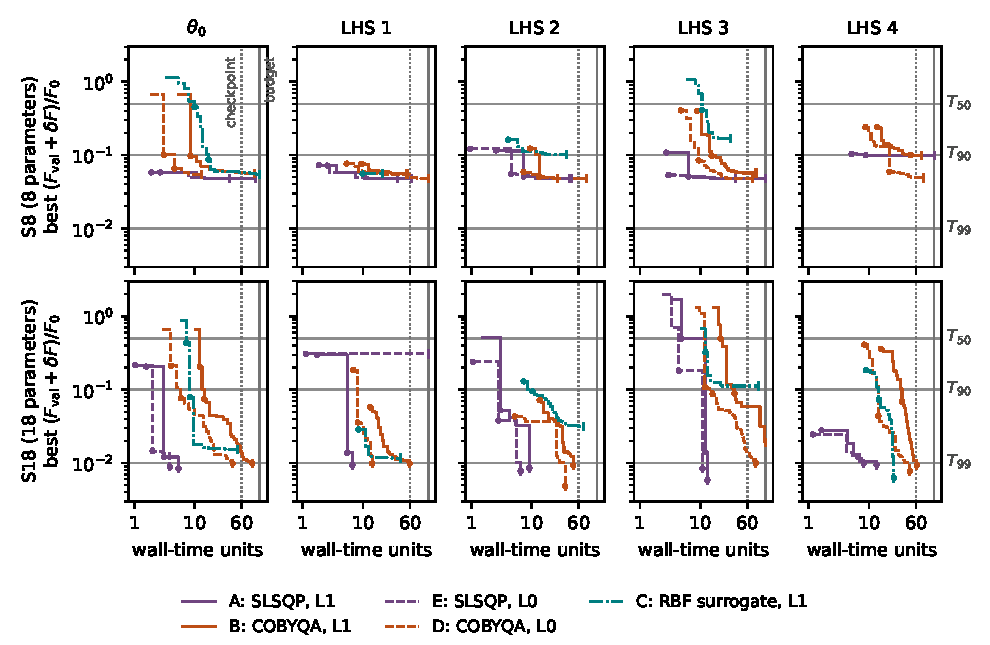
\includegraphics[width=.92\linewidth]{figures/exp2-quality.pdf}
\caption{How fast each method improves. Each panel is one start
($\theta_0$ or Latin-hypercube start LHS~1--4) in one space; each curve is
one method's best credited $(F_{\mathrm{val}}+\delta F)/F_0$ so far, that
is, its validated objective plus the allowance $\delta F$, against charged
wall time (repeat~1, log axes). Lower is better. The labelled grey lines are
the targets $T_{50}$, $T_{90}$ and $T_{99}$, and a dot marks a curve's
first crossing of each; the dotted and solid verticals are the 60-unit
checkpoint and the 120-unit budget. Each curve ends at the run's actual stop
(tick); a missing curve means the run had no credited validation.}
\label{fig:exp2-quality}
\end{figure}

\paragraph{Time to target.}
Figure~\ref{fig:exp2-time} gives the charged time to each target, per
start, and Table~\ref{tab:exp2-time} in Appendix~\ref{sec:exp2-times} lists
the values. In repeat~1, only three crossings occur
after the 60-unit checkpoint, all at $T_{99}$ in S18: two by B and one
by D.

Table~\ref{tab:exp2-ratios} (Appendix~\ref{sec:exp2-times}) gives paired time ratios. A ratio is formed
only when both methods attain the target from that start; no finite ratio
is derived from a censored cell. Wherever both reach a target from the
same start, gradient-based SLSQP gets there sooner than COBYQA at the same
coarse resolution. At L1 (B/A), the geometric-mean ratio is 3.10--3.25 in
S8 and 5.06--7.79 in S18. At L0 (D/E), it is 2.45--2.75 and
3.14--7.20.
All 45 finite optimizer-contrast pairs (by space, target and start) favor
SLSQP, with ratios from 1.46 to 21.5. The coarse mesh shortens the time by
a smaller factor: the geometric-mean E/A ratio is 0.62--0.79 and D/B is
0.45--0.56.

\paragraph{Validation charges.}
Validating every new incumbent makes validation the largest single
charge (Table~\ref{tab:exp2-validation} in Appendix~\ref{sec:exp2-times}). One validation costs a median of
0.87 units over the 3,350 completed validations (range 0.55--1.10), and
validation takes 53\% of all charged time, 2--90\% per run. SLSQP crosses
a target after few validations, but most of its time to a target is
validation; COBYQA at L1 (B) needs more validations, which are a smaller
part of its time. Excluding the validation charges up to each crossing, the
same-resolution geometric means rise to 5.41--5.66 (B/A) and 5.55--5.56
(D/E) in S8, and to 8.84--13.58 and 7.92--15.27 in S18, so the
ratios as charged are conservative for the optimizer contrast. The coarse
mesh cuts the remaining time more, by geometric means of 0.19--0.27 (E/A)
and 0.20--0.23 (D/B), but it does not make validation cheaper, which is why
its overall saving is only 1.3--2.2 times. Against D, the derivative-free
competitor on the coarser mesh, A's lead in S8 comes mostly from
validation: D needs more validated incumbents before it crosses (a median
of six against two), and each costs a full validation. As charged, A is
faster than D by a geometric mean of 1.68--1.83 in S8; excluding the
validation charges it is 1.15--1.16, and two S8 pairs then favor D
(Appendix~\ref{sec:exp2-times}). In S18 A's lead is 2.25--4.32 as charged
and 1.92--3.19 without validation. This contrast changes both the
optimizer and the resolution; one of its 25 pairs is a near tie (0.99, S8
LHS~2 at $T_{90}$: D is 0.75\% faster, within the timing noise between
repeats).

The speed of E has a reliability cost. E never produces a credited
validation from S8 LHS~4. From S18 LHS~1 it reaches $T_{50}$ but
then stalls at $0.28F_0$, missing $T_{90}$ and $T_{99}$. In four
start--target cells, D reaches a target that E misses. A, by contrast,
reaches every target that any method reaches, from every start. C attains
$T_{99}$ only once in S18 and reaches $T_{90}$ from two of five
S8 starts.

\begin{figure}[t]\centering
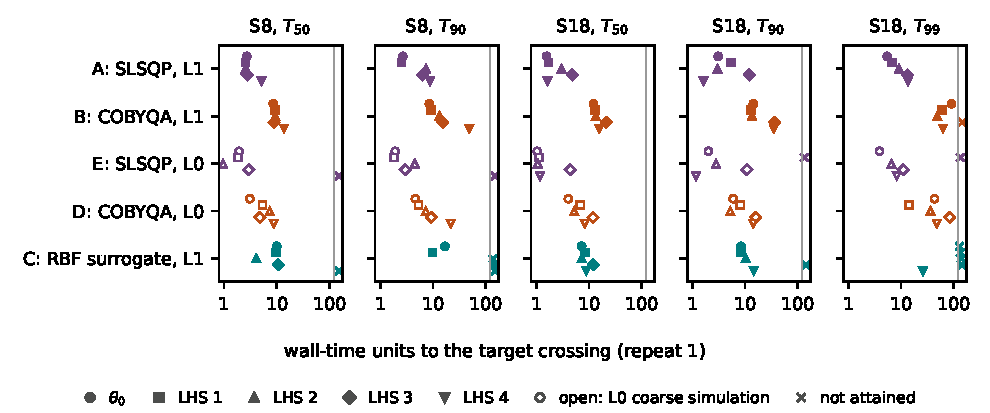
\includegraphics[width=.92\linewidth]{figures/exp2-time-to-target.pdf}
\caption{Charged wall time to each target crossing, repeat~1, for every
target attained by some run. Each row is a method, and each marker shape is
one start, offset vertically so that the same start can be followed across
methods. Filled markers: L1 coarse simulation; open markers: L0; crosses:
not attained within 120 units.}
\label{fig:exp2-time}
\end{figure}

\paragraph{Final refinement.}\label{sec:exp2-refinement}
The preregistered selection takes, for each method and space, the
lowest-$F_{\mathrm{val}}$ feasible design over both repeats, and the
earliest repeat-1 crossing of each attained target. With $\theta_0$ in
each space and identical designs merged, this gives 33 designs. Each
received the six registered checks: the primary L2 validation, L3, a
40-angle grid, Newton tolerance $10^{-12}$, an independently solved grid
shifted by $0.5^\circ$, and held-out currents $0.25$ and $0.75$. The 15
designs with zero stator offsets also received the conforming outer-band
Arkkio check on fresh meshes. All 213 checks completed
(Table~\ref{tab:exp2-refinement} in Appendix~\ref{sec:exp2-times}). These checks qualify the selected
designs only; they do not check each of the study's 111 repeat-1
target crossings.

This is the one deviation from the preregistration noted at the start of
Section~\ref{sec:optimization}: the registered pipeline began by capturing
the closed study on its original host, which had been restarted, so the
refinement used a hash-verified copy of the study outputs on a different
host (Appendix~\ref{sec:protocol-details}). Spatial refinement is the largest change. Over all 33 designs, L3 moves
$F$ by $-4.0\%$ to $+6.3\%$. Over the 25 target crossings alone, the range
is $-4.0\%$ to $+1.1\%$. The largest increase belongs to the overall best
design, D's in S18, whose $F$ rises from $0.0044F_0$ to $0.0047F_0$.
Angular and nonlinear effects are small: the 40-angle and shifted grids
change $F$ by at most $0.11\%$, and the tighter Newton tolerance by less
than $1.1\times10^{-5}$ relative. The conforming estimator gives $1.1\%$ to
$4.4\%$ more ripple than the order-93 coupling on the S8 designs, and
$2.0$--$2.1\%$ more at $\theta_0$. All 25 target crossings still satisfy
their target, allowance included, at L3; the smallest remaining margin is
1.2\% of the target. Every candidate also satisfies the full-current mean
floor in the primary, L3, 40-angle, tight and shifted checks, the closest
by 0.012\%. The refinement therefore confirms the selected crossings and
leaves the time-to-target comparison unchanged. At held-out currents
0.25 and 0.75, part of S18's extra reduction is lost
(Appendix~\ref{sec:exp2-times}).

\section{Post-hoc ablations: adjoint against finite-difference gradients}\label{sec:exp2-fd}
The contrast of Section~\ref{sec:optimization} changes the search strategy
and the gradient source together. Two ablations change only how SLSQP
obtains its gradient, and therefore what the gradient costs. Both were
added after the main outcomes were known and are not part of the
preregistered study; each public protocol was frozen before any of its
runs (Code and data availability). We call the methods of an ablation its
\emph{arms}.

\paragraph{FD-cold.}
FD-cold is the safeguarded SLSQP of A with identical bounds, constraints,
restoration, validation policy, targets, mean floor and stopping rules.
Only the gradients of the objective and of the mean constraint change: they
are forward differences with a step of $10^{-6}$ in each coordinate's
physical unit (metres for the lengths and offsets), reusing the base value,
so one gradient costs $n$ extra coarse forwards, the stencil solves
($n=8$ in S8 and 18 in S18). Each stencil solve is an ordinary coarse
forward on the base point's mesh generation, and like every coarse
forward in the preregistered coarse configuration it starts Newton-cold
(all 40 traces record a cold start). A component whose forward step is
unusable (outside the box, unbuildable or on another mesh generation) takes
the backward step, as 8\% of components did; no gradient was refused.

\paragraph{FD-warm.}
FD-warm, the second arm, is FD-cold except that each stencil solve starts
Newton from its base point's retained converged state on the same mesh
generation, which makes it the stronger finite-difference competitor. In
both arms every solve is charged, and the geometry-constraint Jacobians
remain analytic. Every run is one single-threaded process, so the $n$
stencil solves run one after another and the time ratio is also a ratio
of compute; solving the stencil in parallel would shorten the wall time
per gradient but not its compute.

\paragraph{Controls and estimand.}
Each arm runs with A rerun unchanged in the
same session (A$'$), sharing host, time unit and load, from the five starts
in both spaces on the L1 coarse simulation at 120 units: FD-cold with two
repeats (40 runs), FD-warm with repeat~1 only (20 runs), as its protocol
fixed in advance because FD-cold's repeats had agreed to about 1\% (a
median 1.0\% per primary crossing time) and the estimand uses repeat~1. The
primary estimand is, per start, the repeat-1 time ratio to the primary
target, $T_{90}$ in S8 and $T_{99}$ in S18; a censored cell gives no
finite ratio.

\paragraph{Results.}
Both finite-difference arms and both A$'$ controls reach $T_{50}$ and $T_{90}$
in S8 and all three targets in S18 from all five starts; none
reaches $T_{99}$ in S8, and no cell is censored. Against the stronger
baseline, the adjoint reaches the primary target sooner from every start
(Fig.~\ref{fig:exp2b}): the geometric-mean FD-warm/A$'$ ratio is 1.71 in
S8 (range 1.68--1.77) and 2.70 in S18 (2.62--2.79). Against
cold-started stencils it is 2.47 (2.45--2.52) and 4.11 (3.84--4.33), with
repeat 2 giving 2.49 and 4.04 (Table~\ref{tab:exp2b-ratios}); compared
across sessions, FD-warm takes about 0.72 and 0.68 of FD-cold's time in seconds.
All three arms cross each primary target after the same number of
validations from every start, with one exception at a secondary target
(Appendix~\ref{sec:exp2-times}), so each gap is mainly the cost of the
gradient. Excluding the validation charges up to each crossing, FD-warm/A$'$
becomes 3.23 and 6.10, and FD-cold/A$'$ 5.58 and 10.07.

\begin{figure}[t]\centering
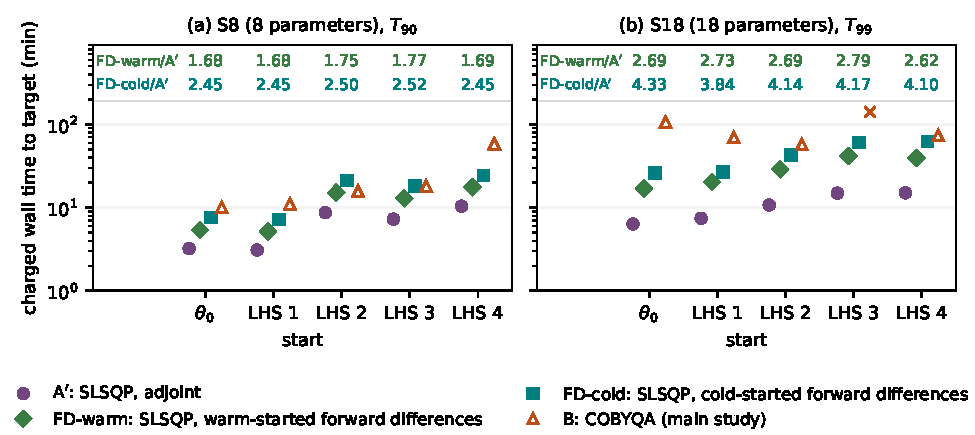
\includegraphics[width=.92\linewidth]{figures/exp2b-per-start.pdf}
\caption{Charged wall time, in minutes, to the primary target from each
start (repeat~1): A$'$ (SLSQP with adjoint gradients, from the FD-warm
session), FD-warm and FD-cold (the same SLSQP with warm- and cold-started
forward-difference gradients, from their own sessions), and B (COBYQA,
main study). Minutes avoid the 3--6\% differences between the sessions'
time units (1 unit is 1.11 to 1.18 minutes). The cross marks the start from
which B did not reach $T_{99}$; it is drawn at B's 120-unit budget. The two
labelled rows above the line give each start's FD-warm/A$'$ and
FD-cold/A$'$ ratio of charged time, each formed within its own session:
FD-warm/A$'$ uses the plotted A$'$, and FD-cold/A$'$ uses the FD-cold
session's A$'$, which is not plotted and agrees with the plotted one
within 4\% (Appendix~\ref{sec:exp2-times}).}
\label{fig:exp2b}
\end{figure}

\paragraph{Gradient factor and optimizer factor.}
Against the main study, B/A $\approx$ (B/FD-warm)(FD-warm/A$'$) splits the
SLSQP-versus-COBYQA ratio into a gradient factor, finite-difference against
adjoint SLSQP, and an optimizer factor, COBYQA against finite-difference
SLSQP. Table~\ref{tab:decomp} gives both splits over the starts where B
attains the primary target (all five in S8; four in S18, where B misses
LHS~3). Over those four starts the FD-warm/A$'$ and FD-cold/A$'$ means are
2.68 and 4.10, against 2.70 and 4.11 over all five starts; the abstract,
introduction and conclusion quote the five-start values.
Of SLSQP's 3.10-fold (S8) and 7.79-fold (S18) advantage over
COBYQA, the gradient accounts for a factor of 1.71--2.47 and 2.68--4.10, and
the optimizer for 1.22--1.76 and 1.91--2.92. The lower gradient factor and
the higher optimizer factor belong to FD-warm, the cheaper finite-difference
baseline; which baseline applies elsewhere depends on whether a solver can
reuse the base point's state. COBYQA was slower than FD-warm from every
start, by as little as 1.01 at S8 LHS~2, whereas against FD-cold it matched
or beat SLSQP from two of five S8 starts (B/FD-cold 0.70 and 0.95). In
seconds, which removes the 3\% difference between the main and FD-warm
sessions' units, B/FD-warm is 1.81 and about 3.0 (per start in
Appendix~\ref{sec:exp2-times}).

\begin{table}[htbp]\centering\small
\caption{The gradient factor and the optimizer factor at the primary
targets: geometric means over the starts where B attains the target (five
in S8, four in S18), each ratio formed within one session's units. The
products close the main study's B/A only approximately, because their
factors come from different sessions.}
\label{tab:decomp}
\begin{tabular}{lrr}\toprule
 & S8, $T_{90}$ & S18, $T_{99}$\\\midrule
Total: COBYQA against adjoint SLSQP (B/A, main study) & 3.10 & 7.79\\
\addlinespace
\multicolumn{3}{l}{\emph{Against warm-started finite differences}}\\
\quad Gradient factor (FD-warm/A$'$) & 1.71 & 2.68\\
\quad Optimizer factor (B/FD-warm) & 1.76 & 2.92\\
\quad Product & 3.02 & 7.82\\
\addlinespace
\multicolumn{3}{l}{\emph{Against cold-started finite differences}}\\
\quad Gradient factor (FD-cold/A$'$) & 2.47 & 4.10\\
\quad Optimizer factor (B/FD-cold) & 1.22 & 1.91\\
\quad Product & 3.02 & 7.82\\
\bottomrule\end{tabular}

\end{table}

\paragraph{Where the time goes.}
Figure~\ref{fig:decomp} splits each arm's mean time to the primary target
into validation, the gradient and the rest (coarse forwards, mesh motion
and optimizer work). The three SLSQP arms spend nearly the same time on
validation and on the rest, because they cross after the same validated
designs: together 5.3--5.4 units in S8 and 8.0--8.1 in S18. The gradient is what
differs. A$'$'s adjoints take about 5\% of its time to the target, 0.30 and
0.51 units, against 4.37 and 14.91 units (45\% and 65\%) for FD-warm's
stencils and 8.72 and 27.47 units (62\% and 77\%) for FD-cold's. A free
gradient would therefore shorten A$'$'s time to the target by only 5--6\%:
the end-to-end ratios are bounded by the validation and coarse forwards
that every arm pays, not by the adjoint. This is why they fall well below
the per-gradient cost ratios of 18--70 below.

\begin{figure}[t]\centering
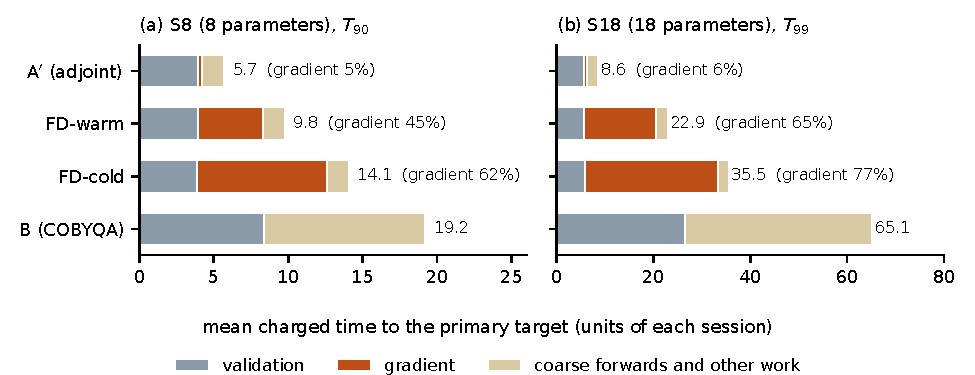
\includegraphics[width=.92\linewidth]{figures/decomp.pdf}
\caption{Mean charged time to the primary target, split into validation
(all validations up to and including the crossing), the gradient (FD-warm's
and FD-cold's stencil solves; A$'$'s adjoints, estimated as the number of
evaluations times the run's mean adjoint charge per evaluation) and the
rest, over the starts of Table~\ref{tab:decomp}. A$'$ is from the FD-warm
session; FD-cold's own A$'$ differs by less than 1\%. B has no gradient;
its rest includes its initial interpolation set. Each bar is in its own
session's unit; the bar labels give the total and, for the SLSQP
arms, the gradient's share of it.}
\label{fig:decomp}
\end{figure}

\paragraph{Gradient cost.}
Costs are in each session's unit, the median cold validation forward (66.66
and 69.09\,s). One adjoint gradient costs A$'$ 0.057 and 0.061 units with
eight and 18 parameters. One finite-difference gradient costs FD-cold 1.90 and
4.25 units, about 0.24 units per cold stencil solve, 33 and 70 times the
adjoint; it costs FD-warm 0.97 and 2.36 units, against 0.054 and 0.059 for
the adjoint in FD-warm's session, 18 and 40 times as much. A warm
stencil solve is charged about half a base coarse forward
(Appendix~\ref{sec:exp2-times}). Two factors shrink the per-gradient ratios. First, every coarse
evaluation costs a coarse forward that both arms pay, 0.216--0.245 units
(Table~\ref{tab:costs}; Appendix~\ref{sec:exp2-times} gives each session's
medians), so an evaluation with a gradient costs FD-cold 7.4 and 14.7
times as much as A$'$. Second, A$'$
requests a gradient at every evaluation, whereas up to the primary
crossing FD-cold and FD-warm request one at a median 83.3\% of their evaluations
in S8 and at 76.9\% and 71.4\% in S18. With both factors the expected
ratios are 6.3 and 11.5 for FD-cold and 3.8 and 6.5 for FD-warm, against the
measured 5.58 and 10.07 and 3.23 and 6.10 once validation is excluded;
Appendix~\ref{sec:exp2-times} discusses the 6--16\% excess.

From 8 to 18 parameters ($n$ grows 2.25-fold) the per-gradient cost ratio
grows 2.2-fold against FD-warm and 2.1-fold against FD-cold, as a cost
proportional to $n$ predicts, but the end-to-end ratio grows only
1.6-fold (1.71 to 2.70) and 1.7-fold (2.47 to 4.11), because validation
and coarse forwards do not grow with $n$. The two spaces also differ in
primary target and in mesh-motion map; at the common target $T_{90}$,
FD-warm/A$'$ is 1.71 in S8 and 2.59 in S18, and FD-cold/A$'$ 2.47 and
3.86. Two spaces do not determine a rate, and we do not extrapolate.

\paragraph{Gradient accuracy.}
FD-cold's L1 gradients pass the max-norm check, and their one component-wise
failure is forward-difference truncation on a small component
(Appendix~\ref{sec:exp2-times}). At the frozen Newton tolerance, warm
stencils are less accurate: FD-warm's max-norm errors are 0.92 to 1.08
times FD-cold's, but its component-wise check fails at all four points, on
small components and once with a reversed sign, from an offset that the
warm stencil objectives share and that a central difference removes
(Appendix~\ref{sec:exp2-times}). The final checks of the selected
designs of all three arms keep every target crossing within its target at
L3, with at least 15\% margin (Appendix~\ref{sec:exp2-times}).